\documentclass[
  journal=pasa,
  manuscript=research-paper, %% or "review"
  year=2021,
  volume=37,
]{cup-journal}

\usepackage{microtype,siunitx,booktabs}

\DeclareRobustCommand{\VAN}[3]{#2}
\let\VANthebibliography\thebibliography
\def\thebibliography{\DeclareRobustCommand{\VAN}[3]{##3}\VANthebibliography}

%%%%% AUTHORS - PLACE YOUR OWN PACKAGES HERE %%%%%
\usepackage{graphicx}	% Including figure files
\usepackage{amsmath}	% Advanced maths commands
\usepackage{amssymb}	% Extra maths symbols
\usepackage{xspace}
\usepackage{upgreek}

%%%%%%%%%%%%%%%%%%%%%%%%%%%%%%%%%%%%%%%%%%%%%%%%%%

%%%%% AUTHORS - PLACE YOUR OWN COMMANDS HERE %%%%%

% COMMENTS
\newcommand{\SB}[1]{{\textcolor{purple}{SB: #1}}}

% STELLAR LABELS
\newcommand{\Teff}{$T_\mathrm{eff}$\xspace}
\newcommand{\logg}{$\log g$\xspace}
\newcommand{\feh}{$\mathrm{[Fe/H]}$\xspace}
\newcommand{\numax}{$\nu_\mathrm{max}$\xspace}
\newcommand{\vmic}{$v_\mathrm{mic}$\xspace}
\newcommand{\vsini}{$v \sin i$\xspace}
\newcommand{\vrad}{$v_\mathrm{rad}$\xspace}

% NAMES
\newcommand{\TheCannon}{\textit{The Cannon}\xspace}
\newcommand{\sme}{\textsc{sme}\xspace}
\newcommand{\marcs}{\textsc{marcs}\xspace}
\newcommand{\Gaia}{\textit{Gaia}\xspace}
\newcommand{\TLF}{\Teff, \logg, and \feh}

% UNITS
\newcommand{\dex}{\,\mathrm{dex}}	% dex
\newcommand{\K}{\,\mathrm{K}}	% dex
\newcommand{\Msol}{\,\mathrm{M_\odot}} % Msol
\newcommand{\kpc}{\,\mathrm{kpc}}	% kpc
\newcommand{\yr}{\,\mathrm{yr}}	% Gyr
\newcommand{\Gyr}{\,\mathrm{Gyr}}	% Gyr
\newcommand{\eV}{\,\mathrm{eV}}	% eV
\newcommand{\Angstroem}{\,\text{\AA}}	% Angstroem
\newcommand{\kms}{\,\mathrm{km\,s^{-1}}}	% km/s
\newcommand{\kpckms}{\,\mathrm{kpc\,km\,s^{-1}}}	% kpc km/s
\newcommand{\kmkmss}{\,\mathrm{km^2\,s^{-2}}}	% km^2/s^2
\newcommand{\kmsMpc}{\,\mathrm{km\,s^{-1}\,Mpc^{-1}}}	% km/s/Mpc

\sisetup{detect-all,separate-uncertainty=true}

\title{The GALAH Survey: Data Release 4}

\author{S. Buder}
\affiliation{Research School of Astronomy \& Astrophysics, Australian National University, Canberra, ACT 2611, Australia}
\affiliation{ARC Centre of Excellence for All Sky Astrophysics in 3 Dimensions (ASTRO 3D), Australia}
\email[S. Buder]{sven.buder@anu.edu.au}

\author{The GALAH Collaboration}
% \alsoaffiliation{Joint first authors}

%\handlingeditor{Excellent E Editor}

\doi{10.1017/pasa.2020.32}

\received {dd Mmm YYYY}
\revised  {dd Mmm YYYY}
\accepted {dd Mmm YYYY}
\published{22 September 2020}

\keywords{
Surveys; the Galaxy; methods: observational; methods: data analysis; stars: fundamental parameters; stars: abundances} %% First letter not capped
% \jel{Q11; Q12; D81; M31}
% \msc{Q14; Q18; E21}
% \abbreviations{
%     BDHS: Bangladesh Demographic and Health Survey, 
%     IDA: Fe-deficiency anaemia, 
%     IFA: Fe-folic acid, 
%     MNP: multiple micronutrient powder, 
%     VAD: vitamin A deficiency
% }

\begin{document}

\begin{abstract}

For each spectrum, we find the best fitting model spectrum by employing a Bayesian framework that takes into account data as well as model uncertainties and can take non-spectroscopic information into account.

We fit all labels (elemental abundances and stellar parameters) simultaneously by using polynomial models created from synthetic spectra with randomly sampled labels for a restricted space in \Teff, \logg, and [Fe/H].

\end{abstract}

\section{INTRODUCTION}

\section{TARGET SELECTION AND OBSERVATION}

\section{REDUCTION}

Outcome of reduction pipeline:
\begin{table}
    \centering
    \caption{Data product 1: FITS files of reduced spectra}
    \label{tab:reduction_fits}
    \begin{tabular}{c|c}
    \hline \hline
    FITS Ext. & Description \\
    \hline
    Ext. 0 & Un-normalised signal~/~counts \\
    Ext. 1 & Normalised signal (by reduction pipeline) \\
    Ext. 2 & Relative uncertainty of signal \\
    Ext. 3 & Subtracted sky signal~/~counts \\
    Ext. 4 & Applied telluric correction \\
    Ext. 5 & Scattered light~/~counts \\
    Ext. 6 & Cross-talk \\
    Ext. 7 & Resolution profile~/~FWHM \\
    \hline
    \end{tabular}
\end{table}

\subsection{Line-spread function} \label{subsec:lsf}

$\texttt{fwhm}\,(\lambda)$, and $\texttt{b}$ reported for each CCD.

\begin{align}
    \exp \left(-0.693147 \vert 2x/\texttt{fwhm}\vert^\texttt{b}\right) \label{eq:lsf}
\end{align}

\section{ANALYSIS}

Our spectroscopic analyses uses a dedicated pipeline for GALAH spectra that implements the latest advancements in the modelling of stellar spectra taking into account for example 1D non-LTE effects and interpolating in the model space with computationally cheap algorithms. To reach agreement with non-spectroscopic information and solve possible degeneracies of the spectroscopic analysis, we run our pipeline in several ways in a Bayesian framework: we first only use spectroscopic information to estimate the most likely set of stellar labels (stellar parameters and abundances) to describe our data. In a second iteration, we also employ non-spectroscopic information as prior information to inform our analysis.

\subsection{Bayesian framework}

\subsubsection{Likelihood functions}

For each part of the spectrum, we can create a model spectrum with flux $f_{m,n} (\vec{l})$ at a given wavelength or pixel $n$ based on a set of stellar labels 
\begin{align}
    \vec{l} \in \{ T_\text{eff}, \log g, \mathrm{[Fe/H]}, v_\mathrm{mic}, v \sin i, \mathrm{[X/Fe]}
    \}
\end{align}

We describe how we actually model $f_{m,n} (\vec{l})$ in Sec.~\ref{subsec:model_spectra}. When confronting each model with with the data, we can calculate a likelihood function. In our case, we assume that the uncertainty of our measurement $\sigma_f$ is Gaussian and therefore can simplify the likelihood function to the $\chi^2$ sum of all pixels $n$
\begin{align} \label{eq:likelihood_spectroscopic}
    P ( f \vert \sigma_{f}, \vec{l} ) = \sum_n \frac{1}{\sqrt{2 \pi} \sigma_{f,n}} \exp \left[ - \frac{\left( f_n - f_{m,n} (\vec{l} ) \right)^2}{2\sigma_{f,n}^2} \right]
\end{align}

When we use additional non-spectroscopic information as prior, we have several choices. If we have asteroseismic information in the form of measurements of $\nu_\text{max}$ available, we can compare that for with a $\nu_{\text{max},m}$ for any specific model, by using the empirical relation \citep{Kjeldsen1995} between $\nu_{\text{max},m}$, \Teff, and \logg
\begin{align}
    \nu_{\text{max},m} = \frac{10^{\log g}}{10^{4.438}\,\mathrm{cm\,s^{-2}}} \sqrt{\frac{T_\text{eff}}{5772\,\mathrm{K}}} \times 3090\,\mathrm{\upmu Hz},
\end{align}
where we define the Solar values for $\nu_\text{max}$ ($3090\,\mathrm{\upmu Hz}$), $T_\mathrm{eff}$ ($5772\,\mathrm{K}$), and $\log g$ ($4.438\,\log{\mathrm{cm\,s^{-2}}}$) as constants.

We can then calculate the likelihood that our model describes the measured $\nu_\text{max}$ and its Gaussian uncertainty $\sigma_{\nu_\text{max}}$ via
\begin{align} 
    P (\nu_\text{max} \vert \sigma_{\nu_\text{max}}, \vec{l}) = \frac{1}{\sqrt{2 \pi} \sigma_{\nu_\text{max}}} \exp \left[ - \frac{\left( \nu_\text{max} - \nu_{\text{max},m} \right)^2}{2\sigma_{\nu_\text{max}}^2} \right].
\end{align}

This allows us to slightly adjust our overall likelihood function to

\begin{align} \label{eq:likelihood_asterospectroscopic}
    P ( f, \nu_\text{max} \vert \sigma_{f}, \sigma_{\nu_\text{max}}, \vec{l} ) = P ( f \vert \sigma_{f}, \vec{l} ) \times P (\nu_\text{max} \vert \sigma_{\nu_\text{max}}, \vec{l})
\end{align}

\SB{Available but not used:
\begin{itemize}
    \item $\varpi$ and its uncertainty from the astrometric solution \citep{Lindegren2021a} of \Gaia eDR3 \citep{Brown2021}, including a zero point correction by \citet{Lindegren2021b}
    \item Optical photometry $G_\text{BP}$, $G$, $G_\text{RP}$ and their uncertainties from \Gaia eDR3 \citep{Brown2021}
    \item Near-infrared photometry $J$, $H$, $K_s$ and their uncertainties from 2MASS \citep{Skrutskie2006}
    \item Infrared photometry $W_1$ - $W_4$ from WISE \citep{Cutri2013}
    \item $\delta_\nu$ and its uncertainty from K2 \citep[][in prep.]{Zinn2020}
\end{itemize}
To be discussed: What do we do, if $\nu_\text{max}$ does not have uncertainties reported?
}

\subsubsection{Prior functions}

We restrict ourselves to the range of reasonable stellar parameters for the analysis with our synthetic spectra, that is $3000 \leq T_\mathrm{eff}~/~\mathrm{K} \leq 8000$, $-0.5 \leq \log (g~/~\mathrm{cm\,s^{-2}}) \leq 5.5$, $v_\text{mic}~/~\mathrm{km\,s^{-1}} > 0$, $v \sin i~/~\mathrm{km\,s^{-1}} > 0$.

With this, we can formulate a prior function $P_s (\vec{l})$ for the purely spectroscopic analysis:
\begin{align}
    P ( \vec{l} ) = \begin{cases}
    1 \quad \text{if within grid limits} \\
    0 \quad \text{otherwise} \\
    \end{cases}
\end{align}

\subsubsection{Posterior functions}

With our likelihood functions and posteriors, we can find combinations of different posterior functions.

If we do only take into account spectroscopic information, we will use the posterior
\begin{align}
    P_s = P ( \vec{l} \vert f, \sigma_f ) = P ( f \vert \vec{l}, \sigma_f ) \times P ( \vec{l} ).
\end{align}

If we take both spectroscopic ($f$, $\sigma_f$) and asteroseismic ($\nu_\text{max}$, $\sigma_{\nu_\text{max}}$) information into account, we will use
\begin{align}\label{eq:posterior}
    P_{sa} = P ( \vec{l} \vert f, \nu_\text{max}, \sigma_f , \sigma_{\nu_\text{max}}) =  P ( f, \nu_\text{max} \vert \sigma_{f}, \sigma_{\nu_\text{max}}, \vec{l} ) ~ P ( \vec{l} ).
\end{align}

\subsection{Creating model spectra} \label{subsec:model_spectra}

In our endeavour to push the limits even further, we are advancing our analysis to fit all 30 elemental abundances and stellar parameters across the full GALAH wavelength range simultaneously with the appropriate model spectra.

To make this computationally feasible, we follow an idea reported by \citet{Rix2016} and create polynomial models for smaller parts of the parameters space from only a limited number of ab initio models \citep[see also][]{Ting2016b}. Our ab initio models are calculated with Spectroscopy Made Easy \citep[\textsc{sme}][]{Valenti1996,Piskunov2017} for the whole wavelength range and all visible atomic and molecular lines for random selections of elemental abundances and stellar parameters within the range of \textsc{marcs} atmospheres \citep{Gustafsson2008}. We then select subsets of these spectra within a restricted space of the three main spectroscopic parameters \Teff, \logg, and [Fe/H]. This idea is comparable to selecting solar twin spectra when analysing the Sun \citep[see e.g.][who applied this idea with tremendous success in the opposite direction]{Nissen2015}. For each subset, we train a quadratic model that correlates stellar flux and labels (stellar parameters and abundances) in the framework of \textit{The Cannon} \citep{Ness2015, Casey2016}. With these models, we can then create model spectra with all lines over the whole wavelength range for any combination of element abundances within this restricted parameter space within less than a second (compared to minutes or hours for physics-driven syntheses). 

In order to confront these model spectra with the GALAH observations, we downgrade the model spectra on-the-fly with the available line-spread functions of each observation (see Sec.~\ref{subsec:lsf}).

\subsubsection{Grid of synthetic spectra} \label{subsubsec:spectrum_grid}

To achieve a self-consistent grid of synthetic spectra, we compute significantly over-sampled synthetic spectra at 10- times higher then the typical GALAH resolution with Spectroscopy Made Easy (\sme). The stellar parameters (\Teff, \logg, \feh, \vmic) and elemental abundances [X/Fe] of all 30 elements are randomly sampled within reasonable limits (see Eq.~\ref{eq:grid_sample_limits}) and fed into \sme to create self-consistent synthetic spectra over the full wavelength range for \marcs atmospheres.

To give an example, we show the limits of the randomly sampled points for the 3D bin with mid point $T_\text{eff} = 5750 \K$, $\log g = 4.5\dex$, and $\mathrm{[Fe/H]} = 0.0\dex$ (see also Fig.~\ref{fig:teff_logg_grid_coverage}):
\begin{align}
    T_\text{eff}~/~\K &\in {5250..5750..6250} \\
    \log g~/~\dex &\in {4.0..4.5..5.0} \\
    \mathrm{[Fe/H]}~/~\dex &\in {-0.5..0.0,0.5} \\
    v_\text{mic}~/~\kms &\in {0.5..1.5..4.0} \\
    v \sin i~/~\kms &\in \text{see Eq.~\ref{eq:vsini}} \\
    \mathrm{[Li/Fe]} &\in {-3.0..1.0..5.0} \\
    \mathrm{[X/Fe]} &\in {-1.0..0.0..1.0}
\end{align}

\begin{figure}[hbt!]
 \centering
 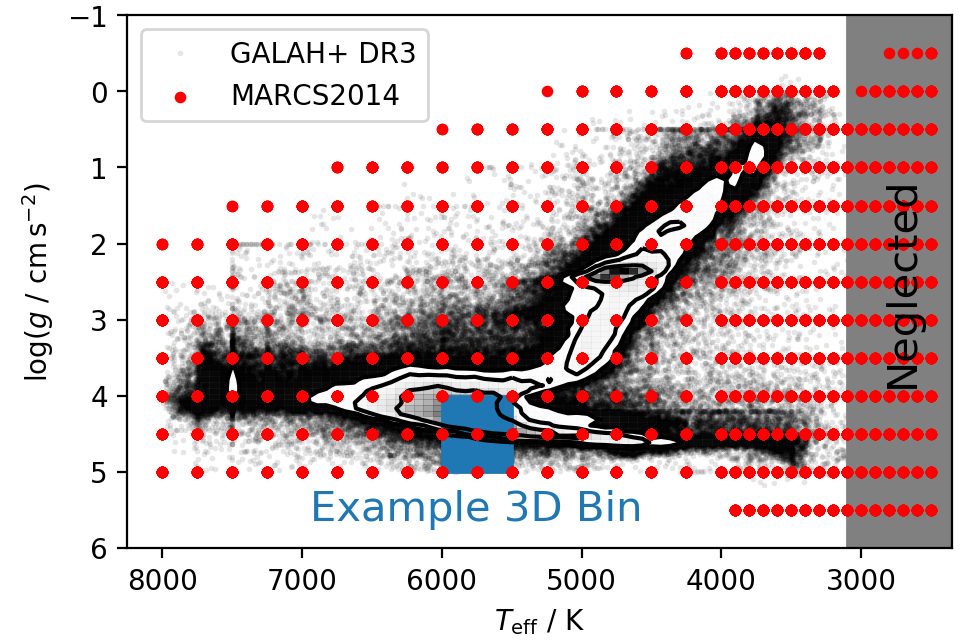
\includegraphics[width=\columnwidth]{figures/teff_logg_grid_coverage.png}
 \caption{Coverage in \Teff and \logg of MARCS2014 grid (red) and GALAH DR3 (black, including density countour). Shown is also an example of one of the 3D bins used to create models with \TheCannon. MARCS grid points \Teff$\leq3100\K$ are neglected throughout GALAH DR4.}
 \label{fig:teff_logg_grid_coverage}
\end{figure}

For each spectrum, we first run a test on all available lines in the GALAH linelist, which is adapted from \citet{Heiter2021} and includes small changes to correct wrong $\log gf$ values for few lines within the GALAH wavelength range. We keep all atomic lines for the final synthesis and restrict the molecular lines to those with \textsc{sme}.depth above 0.001.

Spectra are computed at a resolution of $R = 1,000,000$ on a fine wavelength grid with 60,819 pixels spread over the extended wavelengths $4675.1- 4949.9$, $5624.1-5900.9$, $6424.1-6775.9$, and $7549.1-7925.9 \Angstroem$. We note that these extend significantly beyond the actual GALAH wavelength range.

Default inputs are the grids of 1D \marcs atmospheres \citep[][version 2014]{Gustafsson2008}, which are interpolated for the choice of \Teff, \logg, and \feh. We use grids of non-LTE departure coefficients by \citet{Amarsi2020} for H, Li, C, N, O, Na, Mg, Al, Si, K, Ca, Mn, and Ba. For all, except C, we use the grid, which includes background scattering.

To be able to test that the flux-label correlations found by our subsequent polynomial interpolation are limited to reasonable wavelength ranges, we also calculate one spectrum that is exactly in the middle of the parameter range and additional spectra, where we increase the value of one label at a time (e.g. increase [O/Fe] by $1\dex$) to test the response in the synthetic spectrum.

To save computational power, we compute synthetic spectra without rotational or macroturbulence broadening ($v_\text{mac} = v\sin i = 0\kms$), but save the model continuum flux (\texttt{sme.cmod}) and the specific intensities (\texttt{sme.sint}) as a function of the equal-area midpoints of each equal-area annulus $\mu$ (see Fig.~\ref{fig:sme_mu_output}). These can be integrated after-the fact to sample different \vsini values for the polynomical models (see Sec.\~ref{subsubsec:polynomials}).

\begin{figure}[hbt!]
 \centering
 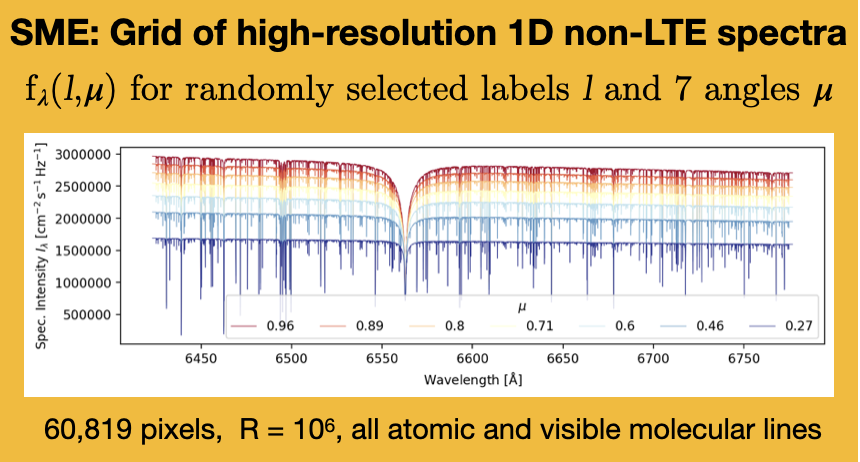
\includegraphics[width=\columnwidth]{figures/sme_grid.png}
 \caption{Example output of \sme for a solar spectrum. Shown are the the specific intensities (\texttt{sme.sint}) as a function of the equal-area midpoints of each equal-area annulus $\mu$.}
 \label{fig:sme_mu_output}
\end{figure}

Our synthetic grid explicitly includes C and N abundances. C was previously included in the analysis of GALAH DR3, but limited to the atomic C line. The analysis thus neglected the molecular absorption features of $\mathrm{C_2}$ and CN at the beginning of CCD1 and end of CCD4, respectively. With the new self-consistent grid, we can however include these features, as they hold valuable information for both C and N, as well as several other features through the molecular equilibrium in stars \citep[see e.g.][]{Ting2018}.

\subsubsection{Polynomial models for a subset} \label{subsubsec:polynomials}

\begin{figure}[hbt!]
 \centering
 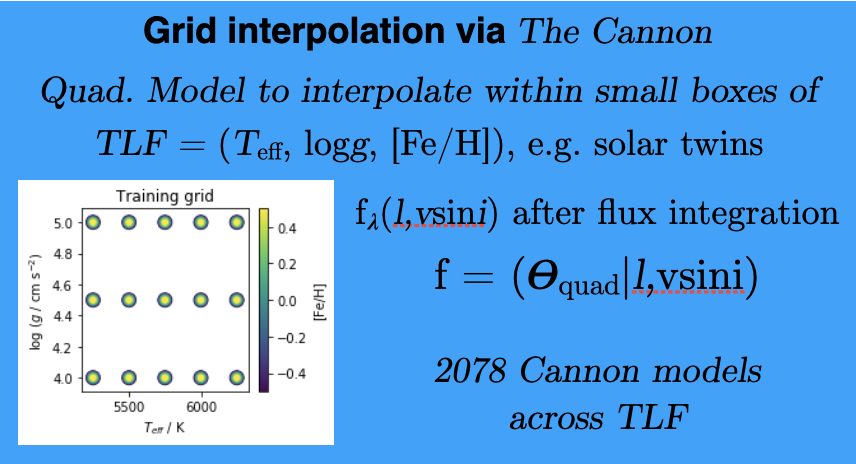
\includegraphics[width=\columnwidth]{figures/cannon_interpolation.png}
 \caption{\SB{Outdated, because this is still not yet showing the actually randomly sampled points!} Explanation of \TheCannon interpolation. Shown are the \Teff and \logg values of the 28x4x6 input spectra for \TheCannon model grid (median $T_\text{eff} = 5750\K$, $\log g = 4.5\dex$, and $\mathrm{[Fe/H]} = 0.0\dex$) that would be used to analyse a Solar spectrum.}
 \label{fig:cannon_interpolation}
\end{figure}

We are training 2067 models for overlapping 3D bins in \Teff, \logg, and \feh.

At this stage, we explicitly include the broadening of spectra because of rotation (\vsini) and sample each of the synthetic spectra over a range of
\begin{align} \label{eq:vsini}
    v \sin i~/~\kms \in \{ 1.5, 3.0, 6.0, 9.0, 12.0, 24.0\}.
\end{align}

The decision for these values was made based on the distribution of \vsini in GALAH+ DR3 and comparison with the grid values used by APOGEE DR16 \citep{Joensson2020}.

Because our interpolation method does not care about the stellar physics behind the correlation of stellar flux and labels, we introduce an intermediate step to verify that the found correlations are at least limited to the wavelength regions where we would expect a reaction to the specific label. This technique is called censoring \citep{Casey2016} or masking \citep{Buder2018}. For our analysis, we explicitly have included perturbations for one label at a time to a median spectrum of the grid. Comparing the median with each of the perturbed spectra at the highest rotational broadening ($v \sin i = 24.0\kms$) allows us to assess which pixels of the synthetic spectra change and only allow the polynomial fitting to find non-zero coefficients for the particular label for exactly these pixels. The idea here is, that coefficients related to Li should for example only be allowed to be non-zero for the Li line. 

\SB{For elements like C, N, O, and Ti, whose molecular bands are visible in the GALAH, a change in either abundance might influence the strength of the other molecular features. We will have to follow this up in more detail!}

\subsubsection{Selecting the best model for the labels at hand}

For each combination of \TLF, we finding \TheCannon's nearest neighbor model via \textsc{scipy} \textsc{cKDTree}.

\SB{Describe here the tests we do to make sure this actually provides a smooth transition between the different labels. Tests of the Cannon models show, that they can reproduce the spectra and their labels within for example $1\K$ \Teff, $0.01\dex$ \logg, and $0.01\dex$ \feh for the grid edges. But more thorough testing is needed}

\subsection{Adjustments to observed spectra} \label{subsec:adjustments_observation}

We make two additional adjustments to the reduced spectra, which come in the form of counts and uncertainty per wavelength, $f_\lambda$ and $\sigma_{f,\lambda}$.

As we compare the observation to model spectra, we do not have to restrict ourselves to an a priory normalisation, but can take into account the residual information on the continuum in parts of the spectra. For each model spectrum that we compare to, we therefore perform a normalisation by fitting a Chebyshev polynomial with outlier clipping to the ratio of model and observation (see Fig.~\ref{fig:ratio_normalisation}). This allows us to both overcome previous shortcomings of the synthetic analysis in GALAH+ DR3 \citep{Buder2021}, which had to be restricted to small wavelength segments and assumed a linear relation for those. Our new approach allows us to properly assess the structure of deep and steep molecular features for cool stars, which dominate spectra of cool stars and carry significant information on \Teff as well as \vrad.

\begin{figure}[hbt!]
 \centering
 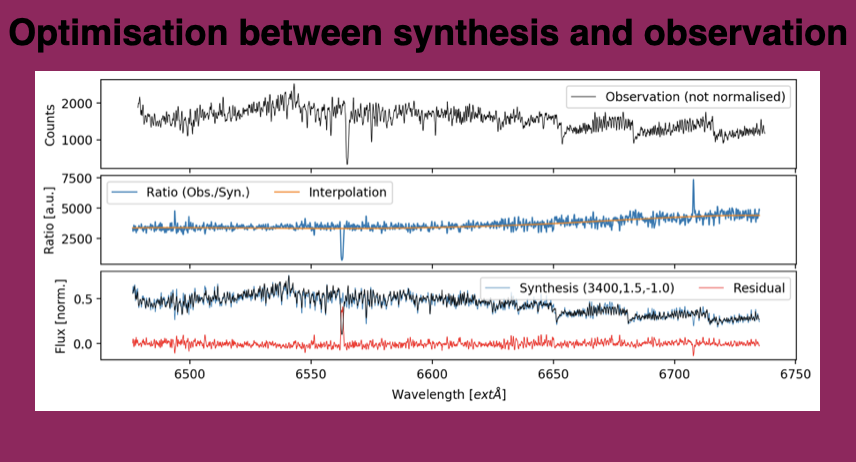
\includegraphics[width=\columnwidth]{figures/ratio_normalisation.png}
 \caption{
 \textbf{Example of normalisation for GALAH DR4 for a model spectrum that is selected during the label optimisation.}
 \textbf{Panel (a):} Observed spectrum (counts) of star 2MASS XYZ.
 \textbf{Panel (b):} Ratio (blue) of observed spectrum and model spectrum as well as Chebychev polynomial fit (orange).
 \textbf{Panel (c):} Normalised observed spectrum (black) compared to the model spectrum (blue). Residuals (red) can then be used as input for the likelihood function.
 }
 \label{fig:ratio_normalisation}
\end{figure}

For each CCD, the reduction has found the most suitable wavelength solution, linking pixels with actual wavelengths, based on the ThXe arc lines. In GALAH DR3 \citep{Buder2021}, we have found several issues for spectra, where not enough ThXe lines could be used to constrain the wavelength solution. Improvements have been made for the new reduction version to improve the number of useful ThXe lines. Two additional pieces of information are, however, unused by the reduction pipeline, namely (i) the telluric lines\footnote{\SB{Check with Janez if that is actually still true!}} that are present throughout GALAH spectra and (ii) the absorption lines of the stellar spectra. Both hold valuable information, as their position (in rest wavelength) is known very well.

The reduction is providing spectra and other parameters in an array of $n$ pixels, that is linked to wavelengths $\lambda_n$ through a linear function
\begin{align} \label{eq:wavelength_solution}
    \lambda (n) = \lambda_0 + n \cdot \Delta_\lambda.
\end{align}
In particular, for each CCD, the pipeline reports $\lambda_0$ as \texttt{cdelt} and $\Delta_\lambda$ as \texttt{CRVAl}.\footnote{\SB{Can we take into account uncertainties on these values through the pipeline? e.g. rms?}}
Because we can directly compare to model spectra with a perfect wavelength solution, we therefore allow these eight values (two for each of the four CCDs) to be fitted by our analysis pipeline.

\SB{Could this be degenarate with \vrad. Could be solved by (i) keeping one CCD fixed or (ii) adding a fit to the telluric lines as well, because we know their dependence on wavelength!}

\subsection{Finding the most likely set of stellar labels}

To find the most set of stellar labels that best describe the data at hand, we need to either (i) maximise/sample the likelihood functions
(Eqs.~\ref{eq:likelihood_spectroscopic} or \ref{eq:likelihood_asterospectroscopic}) or maximise/sample the posterior function (Eq.~\ref{eq:posterior}).

In addition to the parameters included in these functions, we need to optimise the nuisance parameters of \vrad as well as the wavelength solution for the four CCDs (Eq.~\ref{eq:wavelength_solution}).

\SB{MCMC from here}

\section{POST-PROCESSING}

\subsection{Abundance detection or upper limit}

Our pipeline will find the most suitable model and in particular set of abundances for the given observation.

That does, however, not necessarily mean that the abundance of each element is actually well determined, because lines of the element may actually not be detected.

For each element, we therefore run a post-processing routine to estimate if the measured abundance is indeed significant compared to the uncertainty of the spectrum.

For each star, we therefore take the best-fit model and assess the change in the model spectrum when changing one abundance at a time.

\subsection{Flagging of problematic measurements}

Flag if parameters outside of the range of \TheCannon (e.g. \vsini$ > 30 \kms$, see Sec.~\ref{subsubsec:polynomials})

\section{VALIDATION}

\section{CONCLUSIONS}

\section*{Acknowledgements}


% \begin{table*}
% \begin{threeparttable}
% \caption{Identified backscatter from objects in orbit and their properties}\label{satdet}
% \begin{tabular}{ c c c c c c } \toprule
% Satellite\tnote{a}   &NORAD           &Start      &End               &Mean intensity         &RCS\tnote{b}            \\
% name        &ID \#           &time (UT)       &time (UT)             & (Jy/beam)      &($m^{2}$)        \\ \midrule
% BGUSAT      & 41999 &2020-01-31 14:40:09.9  &2020-01-31 14:43:11.9  &1060  &$<$0.1       \\ 
% ISS (ZARYA) & 25544 &2020-01-31 17:17:41.9  &2020-01-31 17:19:00.9  &440  & $>$1.0      \\ 
% MAX VALIER SAT& 42778 &2020-02-03 01:18:16.9  &2020-02-03 01:20:09.9  &650  &0.1 $-$ 1.0       \\
% ISS (ZARYA) &22554 &2020-02-03 01:31:07.9  &2020-02-03 01:33:14.9  &930  &$>$1.0         \\ 
% FLOCK 3P 71 & 42024 &2020-02-01 14:16:22.9& 2020-02-01 14:18:05.9  &330  &$<$0.1       \\ 
% ISS (ZARYA) & 25544 &2020-02-02 02:18:17.9  &2020-02-02 02:20:16.9  &740  &$>$1.0 \\  
% BGUSAT      & 41999 &2020-02-02 02:18:17.9  &2020-02-02 02:20:16.9  &1010  &$<$0.1 \\ \bottomrule
% \end{tabular}
% \begin{tablenotes}
% \item[a] TLE information for predicted trajectories from space-track.org for the epoch of observation: 2020-02-01
% \item[b] Radar Cross Section (RCS) is categorised by space-track.org as: small ($<$0.1); medium (0.1 $<$ RCS $<$ 1.0); and large ($>$1.0)
% \end{tablenotes}
% \end{threeparttable}
% \end{table*}

% PASA uses footnotes, not endnotes. \endnote in this template will behave like \footnote; and \printendnotes will not output anything.
% \printendnotes

\bibliography{bib}

\appendix

% \section{Hospital Anxiety and Depression Scale (Italian Version)}

% \section{Openness to Discuss Cancer in the Family Scale Questionario sulla Comunicazione in Famiglia (Italian Version)}

% \begin{table}[hbt!]
% \centering
% \begin{threeparttable}
% \caption{Predicting approval of one's own house member}\label{tab:predictapproval}
% \begin{tabular}{lSSS}
%   \toprule
%   & {(1)} & {(2)} & {(3)} \\
%   \midrule
%   Religion Match & 0.077\tnote{***} & -0.029 & -0.027 \\
%                   & {(0.014)} & {(0.061)} & {(0.062)} \\
%   \bottomrule
% \end{tabular}
% \begin{tablenotes}[para]
%   \item[]Note: Entries are coefficients from a probit regression model. Robust standard errors in parentheses.
%   \item[***] $p < 0.01$,
%   \item[**] $p < 0.05$,
%   \item[*] $p < 0.1$, two-tailed test.
% \end{tablenotes}
% \end{threeparttable}
% \end{table}


\end{document}
